\documentclass[12pt]{report}

\usepackage{amssymb, fullpage, amsmath, esint}
\usepackage{graphicx}
\usepackage{empheq}


\newtheorem{problem}{Problem}

\newenvironment{solution}[1][\it{Solution}]{\textbf{#1. } }{$\square$}

\graphicspath{ {./} }

\allowdisplaybreaks

\pagestyle{empty}

\def\Z{{\mathbb Z}}
\def\Q{{\mathbb Q}}
\def\C{{\mathbb C}}
\def\R{{\mathbb R}}
\def\N{{\mathbb N}}
\def\eps{{\epsilon}}
\def\O{{\mathcal{O}}}
\newcommand{\floor}[1]{{\left\lfloor#1\right\rfloor}} % Floor function
\newcommand{\ceil}[1]{{\left\lceil#1\right\rceil}} % Ceiling function
\newcommand{\paren}[1]{{\left(#1\right)}} % Parentheses ()
\newcommand{\brac}[1]{{\left\{#1\right\}}} % Curly braces {}
\newcommand{\braces}[1]{{\left[#1\right]}} % Braces []
\newcommand{\abrac}[1]{{\left\langle#1\right\rangle}} % Angle Braces <>
\newcommand{\abs}[1]{{\left|#1\right|}} % Absolute value
\newcommand{\norm}[1]{{\left\|#1\right\|}} % Norm
\newcommand{\eval}[2]{\right|_{#1}^{#2}} % Evaluate

\newcommand{\pp}[2]{\frac{\partial #1}{\partial #2}} % Partial of 1 wrt 2
\newcommand{\ppn}[3]{\frac{\partial^{#1} #2}{\partial #3^{#1}}} % nth Partial of 1 wrt 2
\newcommand{\dd}[2]{\frac{\mathrm{d} #1}{\mathrm{d} #2}} % Partial of 1 wrt 2
\newcommand{\ddn}[3]{\frac{\mathrm{d}^{#1} #2}{\mathrm{d} #3^{#1}}} % nth Partial of 1 wrt 2

\def\ointcc{{\ointctrclockwise}} %counter clockwise contour integral
\def\ointc{{\ointclockwise}} %clockwise contour integral

%dash integral 
\def\Xint#1{\mathchoice
   {\XXint\displaystyle\textstyle{#1}}%
   {\XXint\textstyle\scriptstyle{#1}}%
   {\XXint\scriptstyle\scriptscriptstyle{#1}}%
   {\XXint\scriptscriptstyle\scriptscriptstyle{#1}}%
   \!\int}
\def\XXint#1#2#3{{\setbox0=\hbox{$#1{#2#3}{\int}$}
     \vcenter{\hbox{$#2#3$}}\kern-.5\wd0}}
\def\ddashint{\Xint=}
\def\dashint{\Xint-}

%boxed solution with spacing 0.5cm around equations
\setlength\fboxsep{0.5cm}
\newcommand*\widefbox[1]{\fbox{#1}}


\begin{document}

\large

\begin{center}
 Math 568 Homework 1\\
 Due January 11, 2023\\
 By Marvyn Bailly\\
\end{center}

\normalsize

\hrule

%---------------%
%---Problem 1---%
%---------------%

%--status--$

\begin{problem}
    
\end{problem}

\begin{solution}

    
    \noindent
    Consider the system
    \[ \vec{x}' = \begin{pmatrix}
        2 & -5\\
        1 & -2
    \end{pmatrix}\vec{x}.\]
    \begin{enumerate}
        \item [{\bf Part a:}] Find the eigenvalues and eigenvectors.
        
        \noindent
        To find the eigenvalues, consider
        \[
            \begin{vmatrix}
                2 - \lambda & -5\\
                1 & -2 - \lambda
            \end{vmatrix} = (2 - \lambda)(-2 - \lambda) + 5 = \lambda^2 + 1=0.
        \]
        Thus we have our eigenvalues to be $\lambda_1 = -i$ and $\lambda_2 = i$. Next let's find the eigenvector corresponding to $\lambda_1$. Observe that
        \begin{align*}
            &\begin{pmatrix}
                2 & -5\\
                1 & - 2
            \end{pmatrix}\begin{pmatrix}
                v_1\\
                v_2
            \end{pmatrix} = \lambda_1 \begin{pmatrix}
                v_1\\
                v_2
            \end{pmatrix}\\
            \implies &\begin{pmatrix}
                2v_1 - 5v_2\\
                v_1 - 2v_2
            \end{pmatrix} = \begin{pmatrix}
                -iv_1\\
                -iv_2
            \end{pmatrix}\\
            \implies & \begin{cases}
                2v_1 - 5v_2 = -iv_1\\
                v_1 - 2v_2 = -iv_2
            \end{cases}\\
            \implies &\begin{cases}
                v_1 = 2v_2 - iv_2\\
                v_2 = v_2
            \end{cases}.
        \end{align*}
        Thus lets choose $\vec{v}_1 = \begin{pmatrix}
            2 - i\\
            1
        \end{pmatrix}$. Since the eigenvalues are complex, we know that the eigenvectors are complex conjugates. Thus $\vec{v}_2 = \bar{\vec{v}}_1 =  \begin{pmatrix}
            2 + i\\
            1
        \end{pmatrix}$. Therefore we have the eigenvalues and eigenvectors to be
        \begin{empheq}[box=\widefbox]{align*}
            \lambda_1 &= -i ~~~\text{and}~~~ \vec{v_1} = \begin{pmatrix}
                2 - i\\
                1
            \end{pmatrix}\\
            \lambda_2 &= i ~~~\text{and}~~~ \vec{v_2} = \begin{pmatrix}
                2 + i\\
                1
            \end{pmatrix}
        \end{empheq}

        \item [{\bf Part b:}] Sketch and classify the behavior.
        
        \noindent
        Since the eigenvalues are purely complex. we have a neutrally stable situation with a center critical point. To find the direction of motion, consider the system at various points.
        At $(x_1,x_2) = (1,0)$ we have $x_1' =2$ and $x_2'= 1$. At $(x_1,x_2) = (0,1)$ we have $x_1' = -5$ and $x_2'= -2$. At $(x_1,x_2) = (-1,0)$ we have $x_1' = -2$ and $x_2'= -1$. At $(x_1,x_2) = (0,-1)$ we have $x_1' = 5$ and $x_2'= 2$. Thus we see that the solution trajectories form ellipses with the major axis in the first and third quadrant as shown in the following sketch.
        
            \begin{center}
       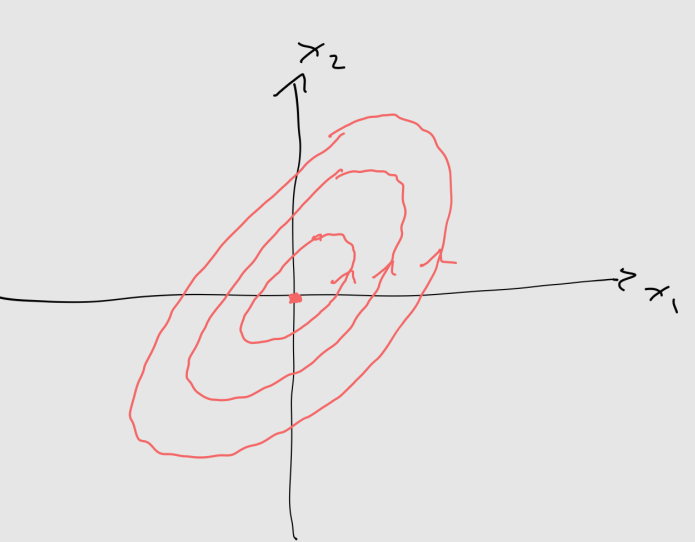
\includegraphics[width=.6\linewidth]{images/1.PNG}
    \end{center}

    \end{enumerate}
\end{solution}

%----------------------------------------------------------------------------------------------------%
%\vskip 20pt
\newpage

%---------------%
%---Problem 2---%
%---------------%

%--status--$

\begin{problem}
    
\end{problem}

\begin{solution}

    
    \noindent
    Consider the system
    \[ \vec{x}' = \begin{pmatrix}
        -1 & -1\\
        0 & -1/4
    \end{pmatrix}\vec{x}.\]
    \begin{enumerate}
        \item [{\bf Part a:}] Find the eigenvalues and eigenvectors.
        
        \noindent
        To find the eigenvalues, consider
        \[
            \begin{vmatrix}
                -1 - \lambda & -1\\
                0 & -1/4 - \lambda
            \end{vmatrix} = (-1 - \lambda)(-1/4 - \lambda) = \lambda^2 + \frac{5}{4}\lambda + \frac{1}{4} = 0.
        \]
        Thus we have our eigenvalues to be $\lambda_1 = - 1/4$ and $\lambda_2 = -1$. Next let's find the eigenvector corresponding to $\lambda_1$. Observe that
        \begin{align*}
            &\begin{pmatrix}
                -1 & -1\\
                0 & -1/4
            \end{pmatrix}\begin{pmatrix}
                v_1\\
                v_2
            \end{pmatrix} = -\frac{1}{4} \begin{pmatrix}
                v_1\\
                v_2
            \end{pmatrix}\\
            \implies & \begin{cases}
                -v_1 - v_2 = - \frac{1}{4}v_1\\
                -\frac{1}{4}v_2 = -\frac{1}{4}v_2
            \end{cases}\\
            \implies &\begin{cases}
                v_1 = - \frac{4}{3}v_2\\
                v_2 = v_2
            \end{cases}.
        \end{align*}
        Thus lets choose $\vec{v}_1 = \begin{pmatrix}
            -4\\
            3
        \end{pmatrix}$.
        Next let's find the eigenvector corresponding to $\lambda_2$. Observe that
        \begin{align*}
            &\begin{pmatrix}
                -1 & -1\\
                0 & -1/4
            \end{pmatrix}\begin{pmatrix}
                v_1\\
                v_2
            \end{pmatrix} = -1 \begin{pmatrix}
                v_1\\
                v_2
            \end{pmatrix}\\
            \implies & \begin{cases}
                -v_1 - v_2 = - v_1\\
                -\frac{1}{4}v_2 = -v_2
            \end{cases}\\
            \implies &\begin{cases}
                v_1 = v_1\\
                v_2 = 0
            \end{cases}.
        \end{align*}
        Thus lets choose $\vec{v}_2 = \begin{pmatrix}
            1\\
            0
        \end{pmatrix}$.
        
        Therefore we have the eigenvalues and eigenvectors to be
        \begin{empheq}[box=\widefbox]{align*}
            \lambda_1 &= -1/4 ~~~\text{and}~~~ \vec{v_1} = \begin{pmatrix}
                -4\\
                3
            \end{pmatrix}\\
            \lambda_2 &= -1 ~~~\text{and}~~~ \vec{v_2} = \begin{pmatrix}
                1\\
                0
            \end{pmatrix}\\
            \vec{x} &= c_1 \vec{v}_1 e^{\lambda_1 t} + c_2 \vec{v}_2 e^{\lambda_2 t}
        \end{empheq}


        \item [{\bf Part b:}] Sketch and classify the behavior.
        
        \noindent
        Since the eigenvalues are real with $\lambda_2 < \lambda_1 < 0$, the behavior of the system is a nodal sink with a stable critical point. Notice that since $\lambda_2 < \lambda_1$, decay occurs most rapidly along $\vec{v_2}$. Therefore the following sketch describes the behavior of solutions in the system. 


            \begin{center}
       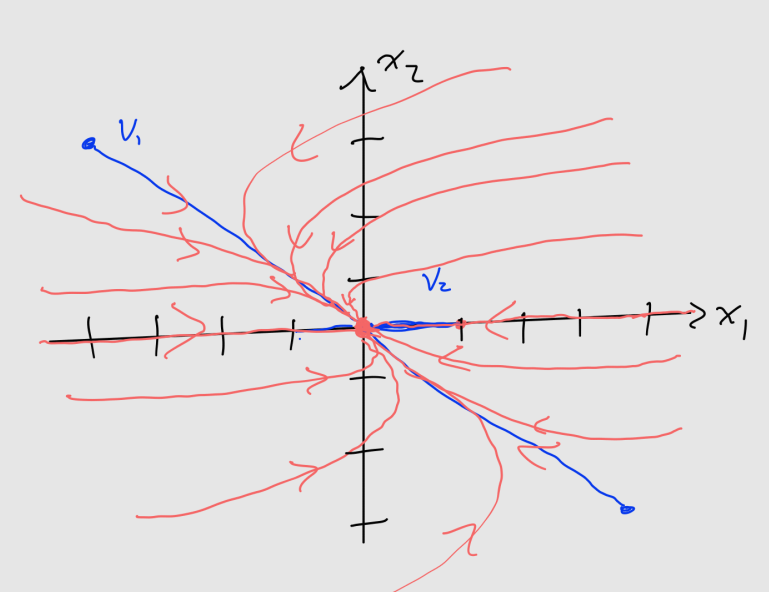
\includegraphics[width=.6\linewidth]{images/2.PNG}
    \end{center}

    \end{enumerate}
\end{solution}
%----------------------------------------------------------------------------------------------------%
%\vskip 20pt
\newpage

%---------------%
%---Problem 3---%
%---------------%

%--status--$

\begin{problem}
    
\end{problem}

\begin{solution}

    
    \noindent
    Consider the system
    \[ \vec{x}' = \begin{pmatrix}
        3 & -4\\
        1 & -1
    \end{pmatrix}\vec{x}.\]
    \begin{enumerate}
        \item [{\bf Part a:}] Find the eigenvalues and eigenvectors.
        
        \noindent
        To find the eigenvalues, consider
        \[
            \begin{vmatrix}
                3 - \lambda & -4\\
                1 & -1 - \lambda
            \end{vmatrix} = \lambda^2 - 2\lambda + 1 = 0
        \]
        Thus we have only one eigenvalue $\lambda = 1$ with multiplicity 2. Next let's find the eigenvector corresponding to $\lambda$. Observe that
        \begin{align*}
            &\begin{pmatrix}
                3 & -4\\
                1 & -1
            \end{pmatrix}\begin{pmatrix}
                v_1\\
                v_2
            \end{pmatrix} = \begin{pmatrix}
                v_1\\
                v_2
            \end{pmatrix}\\
            \implies & \begin{cases}
                3v_1 - 4v_2 = v_1\\
                v_1 - v_2 = v_2
            \end{cases}\\
            \implies &\begin{cases}
                v_1 = 2v_2\\
                v_2 = v_2
            \end{cases}.
        \end{align*}
        Thus lets choose $\vec{v}_1 = \begin{pmatrix}
            2\\
            1
        \end{pmatrix}$. Notice that in this case there is only one linearly independent eigenvector.
        
        To find another eigenvector, lets generate the generalized vector 
        \[ \begin{pmatrix}
            3-\lambda & -4\\
            1 & -1-\lambda
        \end{pmatrix}\vec{\eta} = \begin{pmatrix}
            2\\1
        \end{pmatrix} \implies \begin{cases}
            2\eta_1 -4\eta_2 = 2\\
            1\eta_1 -2\eta_2 = 1
        \end{cases} \implies \begin{cases}
            \eta_1 = 1 + 2\eta_2\\
            \eta_2 = \eta_2
        \end{cases}\] 
        Thus let's let $\vec{\eta} = \begin{pmatrix}
            3\\1
        \end{pmatrix}$.
        Therefore we have the eigenvalue and eigenvector to be
        \begin{empheq}[box=\widefbox]{align*}
            \lambda_1 &= 1 ~~~\text{and}~~~ \vec{v}_1 = \begin{pmatrix}
                2\\
                1
            \end{pmatrix}\\
            \lambda_1 &= 2 ~~~\text{and}~~~ \vec{\eta} = \begin{pmatrix}
                3\\
                1
            \end{pmatrix}\\
            \vec{x} &= c_1 \vec{v}_1e^{\lambda_1 t} + c_2\paren{\vec{v}_1te^{\lambda_1t} + \vec{\eta}e^{\lambda_1 t}}
        \end{empheq}
    
    
    \item [{\bf Part b:}] Sketch and classify the behavior.
        
        \noindent
        Since we have real, positive, equal eigenvalues with only one eigenvector, the system's behavior is an improper node with an unstable critical point. To find the direction of motion, consider the system at $(x_1,x_2) = (0,1)$ which gives $x_1' = -4$ and $x_2' = -1$ and at $(x_1,x_2) = (0,-1)$ gives $x_1' = 4$ and $x_2' = 1$. Thus we can sketch the behavior of the system as following.  

        \begin{center}
            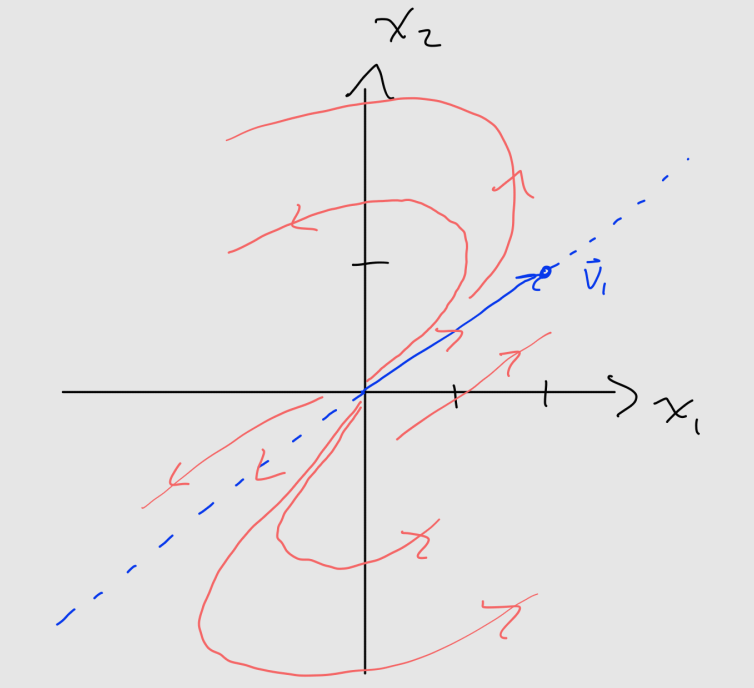
\includegraphics[width=.6\linewidth]{images/3.PNG}
         \end{center}
    \end{enumerate}
\end{solution}
%----------------------------------------------------------------------------------------------------%
%\vskip 20pt
\newpage

%---------------%
%---Problem 4---%
%---------------%

%--status--$

\begin{problem}
    
\end{problem}

\begin{solution}

    
    \noindent
    Consider the system
    \[ \vec{x}' = \begin{pmatrix}
        2 & -5/2\\
        9/5 & -1
    \end{pmatrix}\vec{x}.\]
    \begin{enumerate}
        \item [{\bf Part a:}] Find the eigenvalues and eigenvectors.
        
        \noindent
        To find the eigenvalues, consider
        \[
            \begin{vmatrix}
                2 - \lambda & -5/2\\
                9/5 & -1 - \lambda
            \end{vmatrix} = \lambda^2 - \lambda + 5/2 = 0
        \]
        Thus we have our eigenvalues to be $\lambda_1 = \frac{1}{2} - i\frac{3}{2}$ and $\lambda_2 = \frac{1}{2} + i\frac{3}{2}$. Next let's find the eigenvector corresponding to $\lambda_1$. Observe that
        \begin{align*}
            &\begin{pmatrix}
                2 & -5/2\\
                9/5 & -1
            \end{pmatrix}\begin{pmatrix}
                v_1\\
                v_2
            \end{pmatrix} = \paren{\frac{1}{2} - i\frac{3}{2}} \begin{pmatrix}
                v_1\\
                v_2
            \end{pmatrix}\\
            \implies & \begin{cases}
                \frac{4v_1 - 5v_2}{2} = \frac{x}{2} - i\frac{3x}{2}\\
                \frac{9v_1 - 5v_2}{5} = \frac{y}{2} - i\frac{3y}{2}
            \end{cases}\\
            \implies &\begin{cases}
                v_1 = \frac{5v_2}{6} - i\frac{5v_2}{6}\\
                v_2 = v_2
            \end{cases}.
        \end{align*}
        Thus lets choose $\vec{v}_1 = \begin{pmatrix}
            \frac{5}{6} - i \frac{5}{6}\\
            1
        \end{pmatrix}$. Since the eigenvalues are complex, we know that the eigenvectors are complex conjugates. Thus $\vec{v}_2 = \bar{\vec{v}}_1 = \begin{pmatrix}
            \frac{5}{6} + i \frac{5}{6}\\
            1
        \end{pmatrix}$. Therefore we have the eigenvalues and eigenvectors to be
        \begin{empheq}[box=\widefbox]{align*}
            \lambda_1 &= \frac{1}{2} - i\frac{3}{2} ~~~\text{and}~~~ \vec{v_1} = \begin{pmatrix}
                \frac{5}{6} - i \frac{5}{6}\\
                1
            \end{pmatrix}\\
            \lambda_2 &= \frac{1}{2} + i\frac{3}{2} ~~~\text{and}~~~ \vec{v_2} = \begin{pmatrix}
                \frac{5}{6} + i \frac{5}{6}\\
            1
            \end{pmatrix}
        \end{empheq}

        \item [{\bf Part b:}] Sketch and classify the behavior.
        
        \noindent
        Since the eigenvalues are complex with positive real parts, the system's behavior is a spiral with an unstable equilibrium point. To find the direction of motion, consider the system at $(x_1,x_2) = (1,0)$ which gives $x'_1 = 2$ and $x'_2 = 9/5$. Thus we can sketch the behavior of the system as following. 

        \begin{center}
        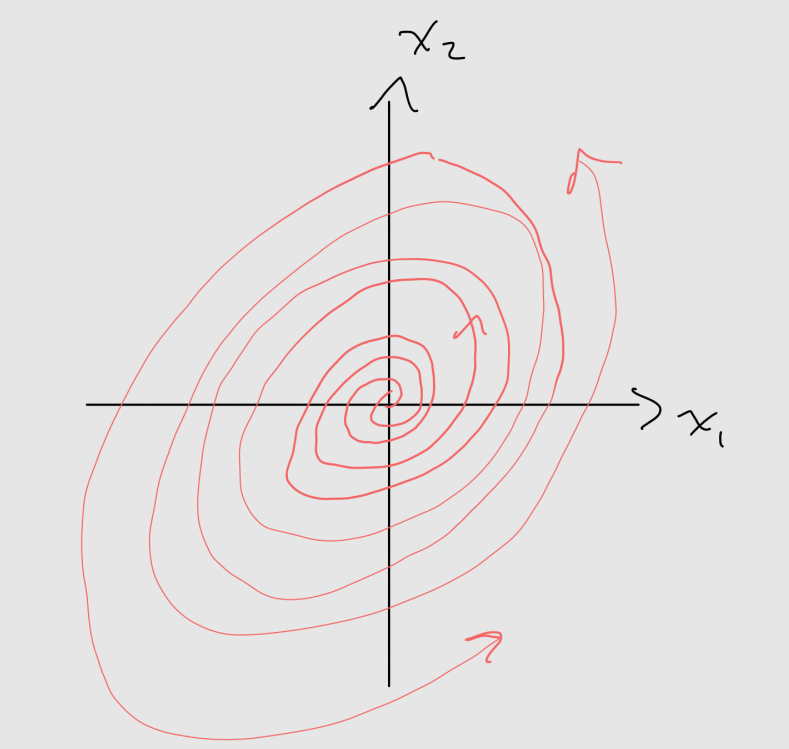
\includegraphics[width=.6\linewidth]{images/4.PNG}
        \end{center}
    \end{enumerate}
\end{solution}
%----------------------------------------------------------------------------------------------------%
%\vskip 20pt
\newpage

%---------------%
%---Problem 5---%
%---------------%

%--status--$

\begin{problem}
    
\end{problem}

\begin{solution}

    
    \noindent
    Consider the system
    \[ \vec{x}' = \begin{pmatrix}
        2 & -1\\
        3 & -2
    \end{pmatrix}\vec{x}.\]
    \begin{enumerate}
        \item [{\bf Part a:}] Find the eigenvalues and eigenvectors.
        
        \noindent
        To find the eigenvalues, consider
        \[
            \begin{vmatrix}
                2 - \lambda & -1\\
                3 & -2 - \lambda
            \end{vmatrix} = \lambda^2 - 1 = 0
        \]
        Thus we have our eigenvalues to be $\lambda_1 = -1$ and $\lambda_2 = 1$. 
        Next let's find the eigenvector corresponding to $\lambda_1$. Observe that
        \begin{align*}
            &\begin{pmatrix}
                2 & -1\\
                3 & -2
            \end{pmatrix}\begin{pmatrix}
                v_1\\
                v_2
            \end{pmatrix} = -1 \begin{pmatrix}
                v_1\\
                v_2
            \end{pmatrix}\\
            \implies & \begin{cases}
                2v_1 - v_2 = -v_1\\
                3v_1 - 2v_2 = -v_2
            \end{cases}\\
            \implies &\begin{cases}
                v_1 = v_2/3\\
                v_2 = v_2
            \end{cases}.
        \end{align*}
        Thus lets choose $\vec{v}_1 = \begin{pmatrix}
            1\\
            3
        \end{pmatrix}$.
        Next let's find the eigenvector corresponding to $\lambda_2$. Observe that
        \begin{align*}
            &\begin{pmatrix}
                2 & -1\\
                3 & -2
            \end{pmatrix}\begin{pmatrix}
                v_1\\
                v_2
            \end{pmatrix} =  \begin{pmatrix}
                v_1\\
                v_2
            \end{pmatrix}\\
            \implies & \begin{cases}
                2v_1 - v_2 = v_1\\
                3v_1 - 2v_2 = v_2
            \end{cases}\\
            \implies &\begin{cases}
                v_1 = v_2\\
                v_2 = v_2
            \end{cases}.
        \end{align*}
        Thus lets choose $\vec{v}_2 = \begin{pmatrix}
            1\\
            1
        \end{pmatrix}$.
        
        Therefore we have the eigenvalues and eigenvectors to be
        \begin{empheq}[box=\widefbox]{align*}
            \lambda_1 &= -1 ~~~\text{and}~~~ \vec{v_1} = \begin{pmatrix}
                1\\
                3
            \end{pmatrix}\\
            \lambda_2 &= 1 ~~~\text{and}~~~ \vec{v_2} = \begin{pmatrix}
                1\\
                1
            \end{pmatrix}\\
            \vec{x} &= c_1 \vec{v}_1 e^{\lambda_1t} + c_2 \vec{v}_2 e^{\lambda_2t}
        \end{empheq}
        
        
        
        \item [{\bf Part b:}] Sketch and classify the behavior.
        
        \noindent
        Since the eigenvalues are real with opposite signs, the behavior is a saddle with an unstable critical point. Since $\lambda_1$ is negative there is decay along $\vec{v}_1$ and since $\lambda_2$ is positive there is growth along $\vec{v}_2$. Thus we can sketch the behavior of the system as follows. 

        \begin{center}
            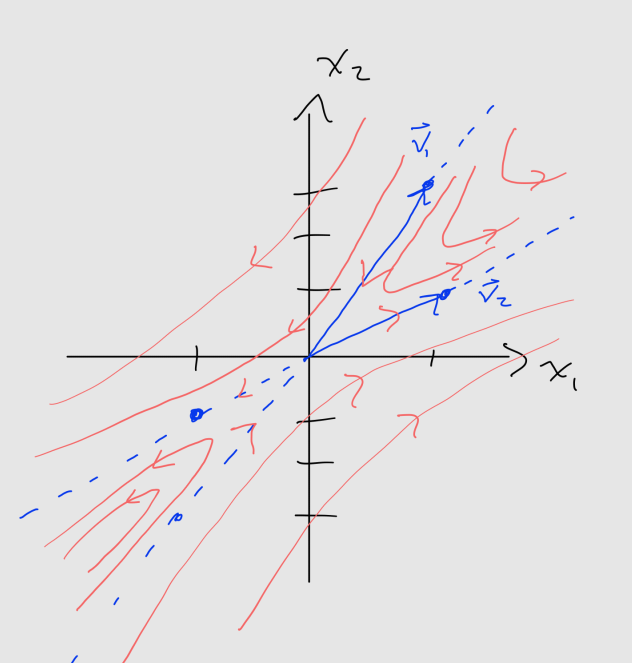
\includegraphics[width=.6\linewidth]{images/5.PNG}
        \end{center}
    \end{enumerate}
\end{solution}
%----------------------------------------------------------------------------------------------------%
%\vskip 20pt
\newpage

%---------------%
%---Problem 6---%
%---------------%

%--status--$

\begin{problem}
    
\end{problem}

\begin{solution}

    
    \noindent
    Consider the system
    \[ \vec{x}' = \begin{pmatrix}
        1 & \sqrt{3}\\
        \sqrt{3} & -1
    \end{pmatrix}\vec{x}.\]
    \begin{enumerate}
        \item [{\bf Part a:}] Find the eigenvalues and eigenvectors.
        
        \noindent
        To find the eigenvalues, consider
        \[
            \begin{vmatrix}
                1 - \lambda & \sqrt{3}\\
                \sqrt{3} & -1 - \lambda
            \end{vmatrix} = \lambda^2 - 4 = 0
        \]
        Thus we have our eigenvalues to be $\lambda_1 = -2$ and $\lambda_2 = 2$. 
        Next let's find the eigenvector corresponding to $\lambda_1$. Observe that
        \begin{align*}
            &\begin{pmatrix}
                1 & \sqrt{3}\\
                \sqrt{3} & -1
            \end{pmatrix}\begin{pmatrix}
                v_1\\
                v_2
            \end{pmatrix} = -2 \begin{pmatrix}
                v_1\\
                v_2
            \end{pmatrix}\\
            \implies & \begin{cases}
                v_1 + \sqrt{3}v_2 = -2v_1\\
                \sqrt{3}v_1 - v_2 = -2v_2
            \end{cases}\\
            \implies &\begin{cases}
                v_1 = -v_2/\sqrt{3}\\
                v_2 = v_2
            \end{cases}.
        \end{align*}
        Thus lets choose $\vec{v}_1 = \begin{pmatrix}
            -1/\sqrt{3}\\
            1
        \end{pmatrix}$.
        Next let's find the eigenvector corresponding to $\lambda_2$. Observe that
        \begin{align*}
            &\begin{pmatrix}
                1 & \sqrt{3}\\
                \sqrt{3} & -1
            \end{pmatrix}\begin{pmatrix}
                v_1\\
                v_2
            \end{pmatrix} = 2 \begin{pmatrix}
                v_1\\
                v_2
            \end{pmatrix}\\
            \implies & \begin{cases}
                v_1 + \sqrt{3}v_2 = 2v_1\\
                \sqrt{3}v_1 - v_2 = 2v_2
            \end{cases}\\
            \implies &\begin{cases}
                v_1 = \sqrt{3}v_2\\
                v_2 = v_2
            \end{cases}.
        \end{align*}
        Thus lets choose $\vec{v}_2 = \begin{pmatrix}
            \sqrt{3}\\
            1
        \end{pmatrix}$.
        
        Therefore we have the eigenvalues and eigenvectors to be
        \begin{empheq}[box=\widefbox]{align*}
            \lambda_1 &= -2 ~~~\text{and}~~~ \vec{v_1} = \begin{pmatrix}
                -1/\sqrt{3}\\
                1  
            \end{pmatrix}\\
            \lambda_2 &= 2 ~~~\text{and}~~~ \vec{v_2} = \begin{pmatrix}
                \sqrt{3}\\
                1
            \end{pmatrix}\\
            \vec{x} &= c_1 \vec{v}_1 e^{\lambda_1t} + c_2 \vec{v}_2 e^{\lambda_2t}
        \end{empheq}
        
        
        
        
        \item [{\bf Part b:}] Sketch and classify the behavior.
        
        \noindent
        Since the eigenvalues are real with opposite signs, the behavior is a saddle with an unstable critical point. Since $\lambda_1$ is negative there is decay along $\vec{v}_1$ and since $\lambda_2$ is positive there is growth along $\vec{v}_2$. Thus we can sketch the behavior of the system as follows.


        \begin{center}
            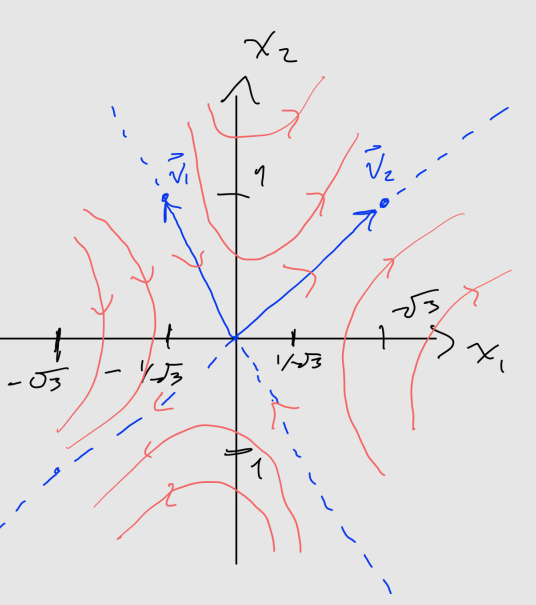
\includegraphics[width=.6\linewidth]{images/6.PNG}
        \end{center}
    \end{enumerate}
\end{solution}
%----------------------------------------------------------------------------------------------------%
%\vskip 20pt
\newpage

%---------------%
%---Problem 7---%
%---------------%

%--status--$

\begin{problem}
    
\end{problem}

\begin{solution}

    \noindent
    Consider the system
    \[ \vec{x}' = \begin{pmatrix}
        3 & -2\\
        2 & -2
    \end{pmatrix}\vec{x}.\]
    \begin{enumerate}
        \item [{\bf Part a:}] Find the eigenvalues and eigenvectors.
        
        \noindent
        To find the eigenvalues, consider
        \[
            \begin{vmatrix}
                3 - \lambda & 2\\
                2 & -2 - \lambda
            \end{vmatrix} = \lambda^2 - \lambda - 2 = 0
        \]
        Thus we have our eigenvalues to be $\lambda_1 = -1$ and $\lambda_2 = 2$. 
        Next let's find the eigenvector corresponding to $\lambda_1$. Observe that
        \begin{align*}
            &\begin{pmatrix}
                3 & -2\\
                2 & -2
            \end{pmatrix}\begin{pmatrix}
                v_1\\
                v_2
            \end{pmatrix} = -1 \begin{pmatrix}
                v_1\\
                v_2
            \end{pmatrix}\\
            \implies & \begin{cases}
                3v_1 - 2v_2 = -v_1\\
                2v_1 - 2v_2 = -v_2
            \end{cases}\\
            \implies &\begin{cases}
                v_1 = v_2\\
                v_2 = 2v_2
            \end{cases}.
        \end{align*}
        Thus lets choose $\vec{v}_1 = \begin{pmatrix}
            1\\
            2
        \end{pmatrix}$.
        Next let's find the eigenvector corresponding to $\lambda_2$. Observe that
        \begin{align*}
            &\begin{pmatrix}
                3 & -2\\
                2 & -2
            \end{pmatrix}\begin{pmatrix}
                v_1\\
                v_2
            \end{pmatrix} = 2 \begin{pmatrix}
                v_1\\
                v_2
            \end{pmatrix}\\
            \implies & \begin{cases}
                3v_1 - 2v_2 = 2v_1\\
                2v_1 - 2v_2 = 2v_2
            \end{cases}\\
            \implies &\begin{cases}
                v_1 = 2v_2\\
                v_2 = v_2
            \end{cases}.
        \end{align*}
        Thus lets choose $\vec{v}_2 = \begin{pmatrix}
            2\\
            1
        \end{pmatrix}$.
        
        Therefore we have the eigenvalues and eigenvectors to be
        \begin{empheq}[box=\widefbox]{align*}
            \lambda_1 &= -1 ~~~\text{and}~~~ \vec{v_1} = \begin{pmatrix}
                1\\
                2  
            \end{pmatrix}\\
            \lambda_2 &= 2 ~~~\text{and}~~~ \vec{v_2} = \begin{pmatrix}
                2\\
                1
            \end{pmatrix}\\
            \vec{x} &= c_1 \vec{v}_1 e^{\lambda_1t} + c_2 \vec{v}_2 e^{\lambda_2t}
        \end{empheq}
        
        
        
        
        \item [{\bf Part b:}] Sketch and classify the behavior.
        
        \noindent
        Since the eigenvalues are real with opposite signs, the behavior is a saddle with an unstable critical point. Since $\lambda_1$ is negative there is decay along $\vec{v}_1$ and since $\lambda_2$ is positive there is growth along $\vec{v}_2$. Thus we can sketch the behavior of the system as follows.

        \begin{center}
            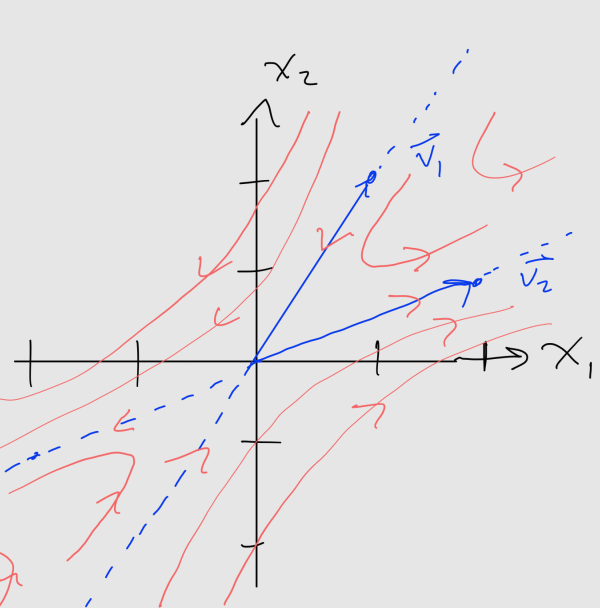
\includegraphics[width=.6\linewidth]{images/7.PNG}
        \end{center}
    \end{enumerate}
\end{solution}
%----------------------------------------------------------------------------------------------------%
%\vskip 20pt
\newpage

%---------------%
%---Problem 8---%
%---------------%

%--status--$

\begin{problem}
    Consider $x' = -(x-y)(1 -x-y)$ and $y' = x(2 +y)$ and plot the solutions. Verify your qualitative dynamics with MATLAB/Python/fortran.
\end{problem}

\begin{solution}

    \noindent
    Consider the nonlinear system $\vec{x}' = F(\vec{x}) = \begin{pmatrix}
        -(x-y)(1 -x-y)\\
        x(2 +y)
    \end{pmatrix}$. First let's find the fixed points which occur when 
    \[
        F(\vec{x}) = \begin{pmatrix}
            -(x-y)(1 -x-y)\\
            x(2 +y)
        \end{pmatrix} = \vec{0} \implies \begin{cases}
            -(x-y)(1 -x-y) = 0\\
            x(2 +y) = 0
        \end{cases}.
    \] 
    Thus we have four fixed points at
    \[ 
        (-2,-2), (0,0), (0,1), ~ \text{and} ~(3,-2).
    \]
    Now to find the local behavior around each fixed point, let's translate our system to that point. After Taylor expanding around the translated point, we can look at the Jacobian of the system evaluated at each point. Note that the general Jacobian for our system is
    \[ 
       J(\vec{x}) = \left(
        \begin{array}{cc}
        2 x-1 & 1-2 y \\
        y+2 & x \\
        \end{array}
        \right).    
    \]

    \noindent 
    Consider fixed point $\vec{x}_0 = (-2,-2)$. Then our Jacobian becomes
    \[ J(\vec{x}_0) = \left(
        \begin{array}{cc}
         -5 & 5 \\
         0 & -2 \\
        \end{array}
        \right).
    \]
    Since the matrix is upper triangular, the eigenvalues are the elements along the main diagonal and thus are given by $\lambda_1 = -5$ and $\lambda_2 = -2$. Next let's find the eigenvectors
    \begin{align*}
        J(\vec{x}_0)\vec{v_1} = \lambda_1 \vec{v_1} \implies \begin{cases}
            -5v_1 + 5v_2 = -5v_1\\
            -2v_2 = -5v_2
        \end{cases} \implies
        \begin{cases}
            v_1 = v_1\\
            v_2 = 0
        \end{cases}\\
        J(\vec{x}_0)\vec{v_2} = \lambda_2 \vec{v_2} \implies \begin{cases}
            -5v_1 + 5v_2 = -2v_1\\
            -2v_2 = -2v_2
        \end{cases} \implies
        \begin{cases}
            v_1 = \frac{5}{3}v_2\\
            v_2 = v_2
        \end{cases}.\\
    \end{align*}
    Thus let's pick the eigenvectors to be $v_1 = \begin{pmatrix}
        1\\0
    \end{pmatrix}$ corresponding to $\lambda_1$ and $v_2 = \begin{pmatrix}
        5\\3
    \end{pmatrix}$ corresponding to $\lambda_2$. Since both eigenvalues are real and negative, we know that this is a sink with a stable critical point. Since $\lambda_1 < \lambda_2$ we have most decay along $v_1$.

    \noindent 
    Consider fixed point $\vec{x}_0 = (0,0)$. Then our Jacobian becomes
    \[ J(\vec{x}_0) = \left(
        \begin{array}{cc}
         -1 & 1 \\
         2 & 0 \\
        \end{array}
        \right).
    \]
    First let's find the eigenvalues.
    \[ 
        \begin{vmatrix}
            -1 - \lambda & 1\\
            2 & -\lambda
        \end{vmatrix} = \lambda^2 + \lambda - 2 = 0
    \]
    Thus are eigenvalues are $\lambda_1 = -2$ and $\lambda_2 = 1$.  Next let's find the eigenvectors
    \begin{align*}
        J(\vec{x}_0)\vec{v_1} = \lambda_1 \vec{v_1} \implies \begin{cases}
            -v_1 + v_2 = -2v_1\\
            2v_1 = -2v_2
        \end{cases} \implies
        \begin{cases}
            v_1 = -v_2\\
            v_2 = v_2
        \end{cases}\\
        J(\vec{x}_0)\vec{v_2} = \lambda_2 \vec{v_2} \implies \begin{cases}
            -v_1 + v_2 = v_1\\
            2v_1 = v_2
        \end{cases} \implies
        \begin{cases}
            v_1 = \frac{1}{2}v_2\\
            v_2 = v_2
        \end{cases}.\\
    \end{align*}
    Thus let's pick the eigenvectors to be $v_1 = \begin{pmatrix}
        -1\\1
    \end{pmatrix}$ corresponding to $\lambda_1$ and $v_2 = \begin{pmatrix}
        2\\1
    \end{pmatrix}$ corresponding to $\lambda_2$. Since both eigenvalues are real and with opposite signs, we know that this is a saddle with an unstable critical point. Since $\lambda_1 < 0 < \lambda_2$ we have decay along $v_1$ and growth along $\lambda_2$.


    \noindent 
    Consider fixed point $\vec{x}_0 = (0,1)$. Then our Jacobian becomes
    \[ J(\vec{x}_0) = \left(
        \begin{array}{cc}
         -1 & -1 \\
         3 & 0 \\
        \end{array}
        \right).
    \]
    First let's find the eigenvalues.
    \[ 
        \begin{vmatrix}
            -1 - \lambda & -1\\
            3 & -\lambda
        \end{vmatrix} = \lambda^2 + \lambda + 3 = 0
    \]
    Thus are eigenvalues are $\lambda_1 = \frac{1}{2}\paren{-1 - i\sqrt{11}}$ and $\lambda_2 = \frac{1}{2}\paren{-1 + i\sqrt{11}}$. Since both eigenvalues are complex and with negative real part, this is a spiral with a stable critical point. To find the direction, let's test $(x_1,x_2) = (0,1)$ in our system which gives $\vec{x}'_1 = -1$ and $\vec{x}'_2 = 0$. Thus the spiral is going counterclockwise. 
    
    
    \noindent 
    Consider fixed point $\vec{x}_0 = (3,-2)$. Then our Jacobian becomes
    \[ J(\vec{x}_0) = \left(
        \begin{array}{cc}
         5 & 5 \\
         0 & 3 \\
        \end{array}
        \right).
    \]
    Since the matrix is upper triangular the eigenvalues are $\lambda_1 = 3$ and $\lambda_2 = 5$. Next let's find the eigenvectors
    \begin{align*}
        J(\vec{x}_0)\vec{v_1} = \lambda_1 \vec{v_1} \implies \begin{cases}
            5v_1 + 5v_2 = 3v_1\\
            3v_2 = 3v_2
        \end{cases} \implies
        \begin{cases}
            v_1 = -\frac{5}{2}v_2\\
            v_2 = v_2
        \end{cases}\\
        J(\vec{x}_0)\vec{v_2} = \lambda_2 \vec{v_2} \implies \begin{cases}
            5v_1 + 5v_2 = 5v_1\\
            3v_2 = 5v_2
        \end{cases} \implies
        \begin{cases}
            v_1 = v_1\\
            v_2 = 0
        \end{cases}.\\
    \end{align*}
    Thus let's pick the eigenvectors to be $v_1 = \begin{pmatrix}
        -5\\2
    \end{pmatrix}$ corresponding to $\lambda_1$ and $v_2 = \begin{pmatrix}
        1\\0
    \end{pmatrix}$ corresponding to $\lambda_2$. Since both eigenvalues are real and postive, we know that this is a node with an unstable critical point. Since $0 > \lambda_1 > \lambda_2$ we have the most growth along $v_2$.

    \noindent
    Combining this information, we get the following sketch that describes the behavior of the system. 
    
    \begin{center}
        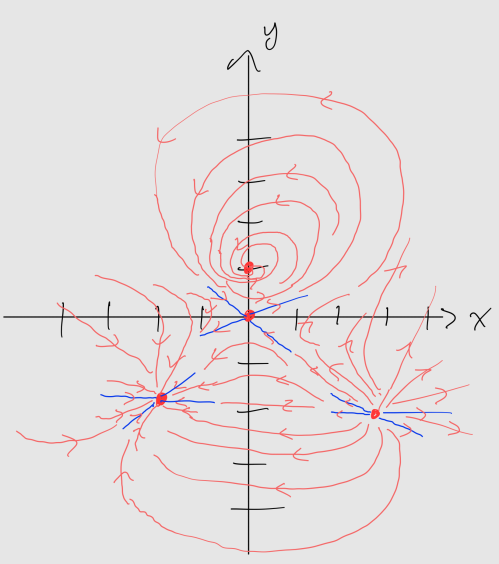
\includegraphics[width=.6\linewidth]{images/8hand.PNG}
    \end{center}

    We can verify this using Mathematica \verb+StreamPlot+ which gives the following plot.

    \begin{center}
       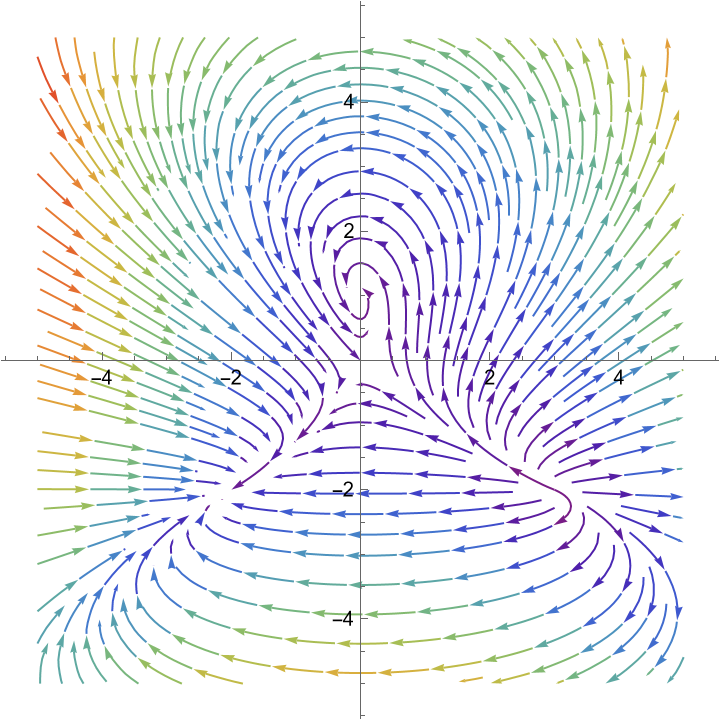
\includegraphics[width=.6\linewidth]{images/8.png}
    \end{center}
    

\end{solution}

%----------------------------------------------------------------------------------------------------%
%\vskip 20pt
\newpage

%---------------%
%---Problem 9---%
%---------------%

%--status--$

\begin{problem}
    Consider $x' = x - y^2$ and $y' = y - x^2$ and plot the solutions. Verify your qualitative dynamics with MATLAB/Python/fortran.
\end{problem}

\begin{solution}

    \noindent
    Consider the nonlinear system $\vec{x}' = F(\vec{x}') = \begin{pmatrix}
        x - y^2\\
        y - x^2
    \end{pmatrix}.$ First let's find the fixed points which occur when
    \[
        F(\vec{x}) = \begin{pmatrix}
            x - y^2\\
            y - x^2
        \end{pmatrix} = \vec{0} \implies \begin{cases}
            x - y^2 = 0\\
            y - x^2 = 0
        \end{cases}.
    \] 
    Thus we have two real fixed points at
    \[ 
        (0,0) ~\text{and}~ (1,1).
    \]
    Now to find the local behavior around each fixed point, let's translate our system to that point. After Taylor expanding around the translated point, we can look at the Jacobian of the system evaluated at each point. Note that the general Jacobian for our system is
    \[ 
        J(\vec{x}) = \begin{pmatrix}
            1 & -2y\\
            -2x & 1
        \end{pmatrix}.
    \]
    
    \noindent
    Consider the fixed point $\vec{x}_0 = (0,0)$. then our Jacobian becomes
    \[ 
        \begin{pmatrix}
            1 & 0\\
            0 & 1
        \end{pmatrix},
    \]
    which is the identity matrix. We know that the identity matrix has eigenvalues $\lambda = 1$ with multiplicity 2 and eigenvectors $v_1 = \begin{pmatrix}
        1 \\ 0
    \end{pmatrix}$ and $v_2 = \begin{pmatrix}
        0 \\ 1
    \end{pmatrix}$. Since we have real, positive, and equal eigenvalues with two linear independent eigenvectors this is a proper node with an unstable critical point. 


    \noindent
    Consider the fixed point $\vec{x}_0 = (1,1)$. then our Jacobian becomes
    \[ 
        \begin{pmatrix}
            1 & -2\\
            -2 & 1
        \end{pmatrix}.
    \]
    First lets find the eigenvalues
    \[ 
        \begin{vmatrix}
            1 - \lambda & -2\\
            -2 & 1 - \lambda
        \end{vmatrix} = \lambda^2 - 2 \lambda - 3 = 0,
    \]
    thus are eigenvalues are $\lambda_1 = -1$ and $\lambda_2 = 3$. Now let's find the eigenvectors.
    \begin{align*}
        J(\vec{x}_0)\vec{v_1} = \lambda_1 \vec{v_1} \implies \begin{cases}
            v_1 - 2v_2 = -v_1\\
            -2v_1 + v_2 = -v_2
        \end{cases} \implies
        \begin{cases}
            v_1 = v_2\\
            v_2 = v_2
        \end{cases}\\
        J(\vec{x}_0)\vec{v_2} = \lambda_2 \vec{v_2} \implies \begin{cases}
            v_1 - 2v_2 = 3v_1\\
            -2v_1 + v_2 = 3v_2
        \end{cases} \implies
        \begin{cases}
            v_1 = -v_2\\
            v_2 = v_2
        \end{cases}.\\
    \end{align*}
    Thus let's pick the eigenvectors to be $v_1 = \begin{pmatrix}
        1\\1
    \end{pmatrix}$ corresponding to $\lambda_1$ and $v_2 = \begin{pmatrix}
        -1\\1
    \end{pmatrix}$ corresponding to $\lambda_2$. Since both eigenvalues are real with $\lambda_1 < 0 < \lambda_2$ we have a saddle with an unstable critical point with decay along $\vec{v}_1$ and growth along $\vec{v}_2$. 

    \noindent
    Combining this information, we get the following sketch that describes the behavior of the system. 
    
    \begin{center}
        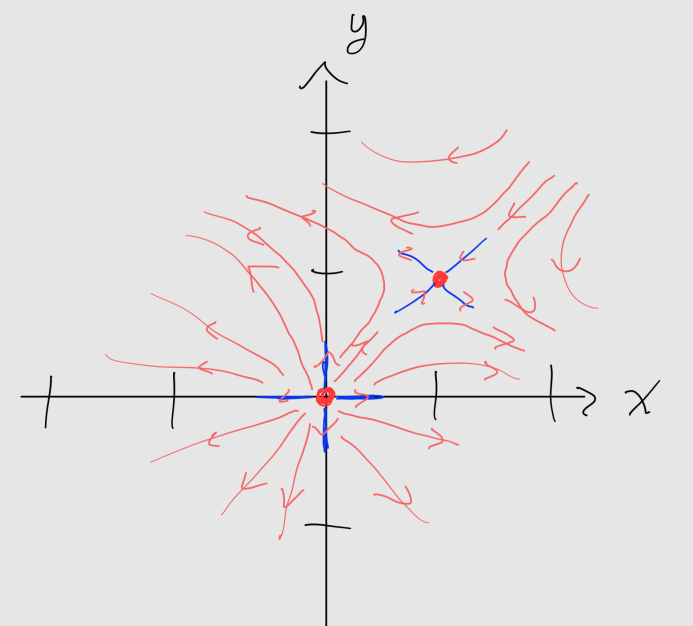
\includegraphics[width=.6\linewidth]{images/9hand.PNG}
    \end{center}

    \noindent
    We can verify this using Mathematica \verb+StreamPlot+ which gives the following plot.

    \begin{center}
       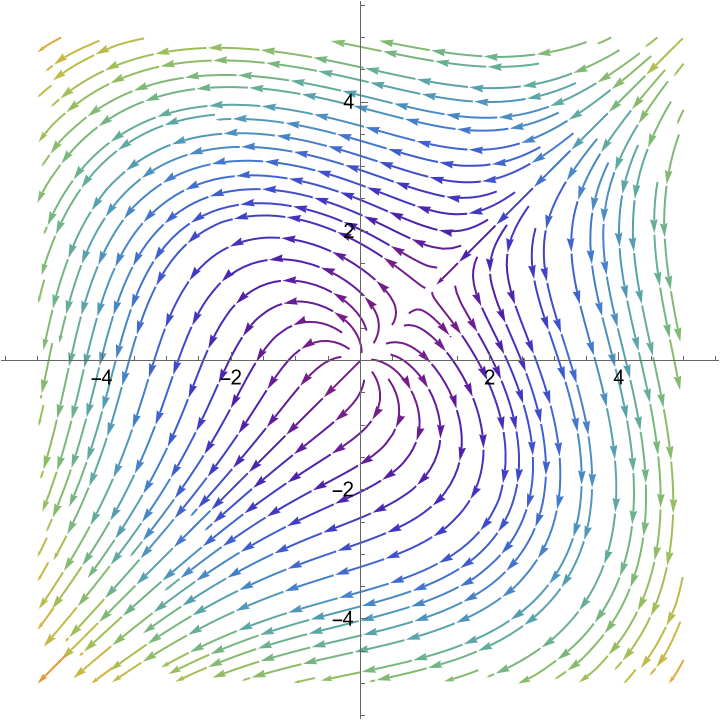
\includegraphics[width=.6\linewidth]{images/9.png}
    \end{center}


\end{solution}

%----------------------------------------------------------------------------------------------------%
%\vskip 20pt
\newpage

%---------------%
%---Problem 10---%
%---------------%

%--status--$

\begin{problem}
    Consider $x' = (2+x)(y-x)$ and $y' = (4-x)(y+x)$ and plot the solutions. Verify your qualitative dynamics with MATLAB/Python/fortran.
\end{problem}

\begin{solution}

    \noindent
    Consider the nonlinear system $\vec{x}' = F(\vec{x}') = \begin{pmatrix}
        (2 + x)(y - x)\\
        (4 - x)(y + x)
    \end{pmatrix}.$ First let's find the fixed points which occur when
    \[
        F(\vec{x}) = \begin{pmatrix}
            (2 + x)(y - x)\\
            (4 - x)(y + x)
        \end{pmatrix} = \vec{0} \implies \begin{cases}
            (2 + x)(y - x) = 0\\
            (4 - x)(y + x) = 0
        \end{cases}.
    \]
    Thus we have three fixed points at
    \[ 
        (-2,2), (0,0) ~\text{and}~ (4,4).
    \]
    Now to find the local behavior around each fixed point, let's translate our system to that point. After Taylor expanding around the translated point, we can look at the Jacobian of the system evaluated at each point. Note that the general Jacobian for our system is
    \[ 
        \begin{pmatrix}
            -2-2x+y & 2 + x\\
            4 - 2x - y &  4 - x
        \end{pmatrix}.
    \]
    Consider the fixed point $\vec{x}_0 = (-2,2)$. Then our Jacobian becomes
    \[ 
        \begin{pmatrix}
            4 & 0 \\
            6 & 6  
        \end{pmatrix}.
    \]
    First lets find the eigenvalues,
    \[ 
        \begin{vmatrix}
            4 - \lambda & 0 \\
            6 & 6 - \lambda 
        \end{vmatrix} = \lambda^2 - 10\lambda + 24 = 0.
    \]
    Thus are eigenvalues are $\lambda_1 = 4$ and $\lambda_2 = 6$. Now let's find the eigenvectors.
    \begin{align*}
        J(\vec{x}_0)\vec{v_1} = \lambda_1 \vec{v_1} \implies \begin{cases}
            4v_1 = 4v_1\\
            6v_1 + 6v_2 = 4v_2
        \end{cases} \implies
        \begin{cases}
            v_1 = v_1\\
            v_2 = -3v_1
        \end{cases}\\
        J(\vec{x}_0)\vec{v_2} = \lambda_2 \vec{v_2} \implies \begin{cases}
            4v_1 = 6v_1\\
            6v_1 + 6v_2 = 6v_2
        \end{cases} \implies
        \begin{cases}
            v_1 = 0\\
            v_2 = v_2
        \end{cases}.\\
    \end{align*}
    Thus let's pick the eigenvectors to be $v_1 = \begin{pmatrix}
        -1\\3
    \end{pmatrix}$ corresponding to $\lambda_1$ and $v_2 = \begin{pmatrix}
        0\\1
    \end{pmatrix}$ corresponding to $\lambda_2$. Since both eigenvalues are real with $0<\lambda_1 < \lambda_2$ we have a node with an unstable critical point and the most growth along $\vec{v}_2$. 



    \noindent
    Consider the fixed point $\vec{x}_0 = (0,0)$. Then our Jacobian becomes
    \[ 
        \begin{pmatrix}
            -2 & 2 \\
            4 & 4  
        \end{pmatrix}.
    \]
    First lets find the eigenvalues,
    \[ 
        \begin{vmatrix}
            -2 - \lambda & 2 \\
            4 & 4 - \lambda 
        \end{vmatrix} = \lambda^2 - 2\lambda - 16 = 0.
    \]
    Thus are eigenvalues are $\lambda_1 = 1 - \sqrt{17}$ and $\lambda_2 = 1 + \sqrt{17}$. Now let's find the eigenvectors.
    \begin{align*}
        J(\vec{x}_0)\vec{v_1} = \lambda_1 \vec{v_1} \implies \begin{cases}
            -2v_1 + 2v_2 = (1 - \sqrt{17})v_1\\
            4v_1 + 4v_2 = (1 - \sqrt{17})v_2
        \end{cases} \implies
        \begin{cases}
            v_1 = \paren{\frac{-3}{4} + \frac{\sqrt{17}}{4}}v_1\\
            v_2 = v_2
        \end{cases}\\
        J(\vec{x}_0)\vec{v_2} = \lambda_2 \vec{v_2} \implies \begin{cases}
            -2v_1 + 2v_2 = (1 + \sqrt{17})v_1\\
            4v_1 + 4v_2 = (1 + \sqrt{17})v_2
        \end{cases} \implies
        \begin{cases}
            v_1 = \paren{\frac{-3}{4} - \frac{\sqrt{17}}{4}}v_1\\
            v_2 = v_2
        \end{cases}.\\
    \end{align*}
    Thus let's pick the eigenvectors to be $v_1 = \begin{pmatrix}
        \frac{-3}{4} - \frac{\sqrt{17}}{4}\\1
    \end{pmatrix}$ corresponding to $\lambda_1$ and $v_2 = \begin{pmatrix}
        \frac{-3}{4} + \frac{\sqrt{17}}{4}\\1
    \end{pmatrix}$ corresponding to $\lambda_2$. Since both eigenvalues are real with $\lambda_1 < 0 < \lambda_2$ we have a saddle with an unstable critical point and growth along $\vec{v}_2$ and decay along $\vec{v}_1$. 

    \noindent
    Consider the fixed point $\vec{x}_0 = (4,4)$. Then our Jacobian becomes
    \[ 
        \begin{pmatrix}
            -6 & 6 \\
            8 & 0  
        \end{pmatrix}.
    \]
    First lets find the eigenvalues,
    \[ 
        \begin{vmatrix}
            -6 - \lambda & 6 \\
            8 & - \lambda 
        \end{vmatrix} = \lambda^2 + 6\lambda + 48 = 0.
    \]
    Thus are eigenvalues are $\lambda_1 = -3 + i\sqrt{39}$ and $\lambda_2 = -3 - i\sqrt{39}$. Since both are eigenvalues are complex with negative real part, this is a spiral with a stable critical point. We can find the direction of motion by observing the other behavior of the other critical points. Thus combining all our information we get the following sketch that describes the behavior of the system. 
    \begin{center}
        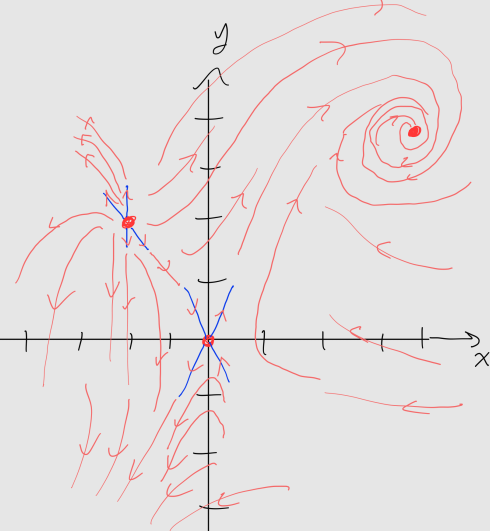
\includegraphics[width=.6\linewidth]{images/10hand.PNG}
    \end{center}


    \noindent
    We can verify this using Mathematica \verb+StreamPlot+ which gives the following plot.
    \begin{center}
       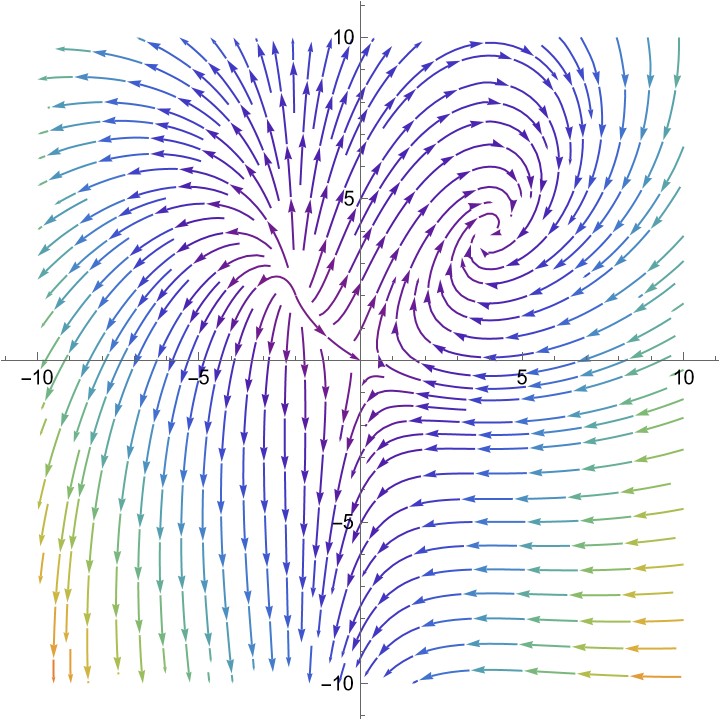
\includegraphics[width=.6\linewidth]{images/10.png}
    \end{center}

\end{solution}

\end{document}